%% abtex2-modelo-relatorio-tecnico.tex, v-1.7.1 laurocesar
%% Copyright 2012-2013 by abnTeX2 group at http://abntex2.googlecode.com/ 
%%
%% This work may be distributed and/or modified under the
%% conditions of the LaTeX Project Public License, either version 1.3
%% of this license or (at your option) any later version.
%% The latest version of this license is in
%%   http://www.latex-project.org/lppl.txt
%% and version 1.3 or later is part of all distributions of LaTeX
%% version 2005/12/01 or later.
%%
%% This work has the LPPL maintenance status `maintained'.
%% 
%% The Current Maintainer of this work is the abnTeX2 team, led
%% by Lauro César Araujo. Further information are available on 
%% http://abntex2.googlecode.com/
%%
%% This work consists of the files abntex2-modelo-relatorio-tecnico.tex,
%% abntex2-modelo-include-comandos and abntex2-modelo-references.bib
%%

% ------------------------------------------------------------------------
% ------------------------------------------------------------------------
% abnTeX2: Modelo de Relatório Técnico/Acadêmico em conformidade com 
% ABNT NBR 10719:2011 Informação e documentação - Relatório técnico e/ou
% científico - Apresentação
% ------------------------------------------------------------------------ 
% ------------------------------------------------------------------------

% Alterado por Rodrigo Campiolo para apresentação de relatórios na disciplina
% de Redes de Computadores II do Bacharelado em Ciência da Computação da UTFPR-CM.


\documentclass[
	% -- opções da classe memoir --
	12pt,				% tamanho da fonte
	%openright,			% capítulos começam em pág ímpar (insere página vazia caso preciso)
	oneside,   	        % para impressão em verso e anverso use twoside. Oposto a oneside
	a4paper,			% tamanho do papel. 
	% -- opções da classe abntex2 --
	%chapter=TITLE,		% títulos de capítulos convertidos em letras maiúsculas
	%section=TITLE,		% títulos de seções convertidos em letras maiúsculas
	%subsection=TITLE,	% títulos de subseções convertidos em letras maiúsculas
	%subsubsection=TITLE,% títulos de subsubseções convertidos em letras maiúsculas
	% -- opções do pacote babel --
	english,			% idioma adicional para hifenização
	french,				% idioma adicional para hifenização
	spanish,			% idioma adicional para hifenização
	brazil,				% o último idioma é o principal do documento
	]{pacotes/abntex2}


% ---
% PACOTES
% ---

% ---
% Pacotes fundamentais 
% ---
\usepackage{cmap}				% Mapear caracteres especiais no PDF
\usepackage{lmodern}			% Usa a fonte Latin Modern
\usepackage[T1]{fontenc}		% Selecao de codigos de fonte.
\usepackage[utf8]{inputenc}		% Codificacao do documento (conversão automática dos acentos)
\usepackage{indentfirst}		% Indenta o primeiro parágrafo de cada seção.
\usepackage{color}				% Controle das cores
\usepackage{graphicx}			% Inclusão de gráficos
% ---

% ---
% Pacotes adicionais, usados no anexo do modelo de folha de identificação
% ---
\usepackage{multicol}
\usepackage{multirow}
% ---
	
% ---
% Pacotes adicionais, usados apenas no âmbito do Modelo Canônico do abnteX2
% ---
\usepackage{lipsum}				% para geração de dummy text
% ---

% ---
% Pacotes de citações
% ---
\usepackage[brazilian,hyperpageref]{backref}	 % Paginas com as citações na bibl
\usepackage[alf]{pacotes/abntex2cite}	% Citações padrão ABNT
\usepackage{comment}
% --- 
% CONFIGURAÇÕES DE PACOTES
% --- 

% ---
% Configurações do pacote backref
% Usado sem a opção hyperpageref de backref
\renewcommand{\backrefpagesname}{Citado na(s) página(s):~}
% Texto padrão antes do número das páginas
\renewcommand{\backref}{}
% Define os textos da citação
\renewcommand*{\backrefalt}[4]{
	\ifcase #1 %
		Nenhuma citação no texto.%
	\or
		Citado na página #2.%
	\else
		Citado #1 vezes nas páginas #2.%
	\fi}%
% ---

% ---
% Informações de dados para CAPA e FOLHA DE ROSTO
% ---
\titulo{Título da atividade \\ prática}
\autor{Hendrick \\João Victor Briganti\\ Luiz Gustavo Takeda}
\local{Campo Mourão}
\data{Outubro / 2024}
\instituicao{%
  Universidade Tecnológica Federal do Paraná -- UTFPR
  \par
  Departamento Acadêmico de Computação -- DACOM
  \par
  Bacharelado em Ciência da Computação -- BCC
}
\tipotrabalho{Relatório técnico}
% O preambulo deve conter o tipo do trabalho, o objetivo, 
% o nome da instituição e a área de concentração 
\preambulo{Relatório técnico de atividade prática solicitado pelo professor Rodrigo Campiolo na disciplina de Redes de Computadores II do Bacharelado em Ciência da Computação da Universidade Tecnológica Federal do Paraná.}
% ---

% ---
% Configurações de aparência do PDF final

% alterando o aspecto da cor azul
\definecolor{blue}{RGB}{41,5,195}

% informações do PDF
\makeatletter
\hypersetup{
     	%pagebackref=true,
		pdftitle={\@title}, 
		pdfauthor={\@author},
    	pdfsubject={\imprimirpreambulo},
	    pdfcreator={LaTeX with abnTeX2},
		pdfkeywords={abnt}{latex}{abntex}{abntex2}{relatório técnico}, 
		colorlinks=true,       		% false: boxed links; true: colored links
    	linkcolor=blue,          	% color of internal links
    	citecolor=blue,        		% color of links to bibliography
    	filecolor=magenta,      		% color of file links
		urlcolor=blue,
		bookmarksdepth=4
}
\makeatother
% --- 

% --- 
% Espaçamentos entre linhas e parágrafos 
% --- 

% O tamanho do parágrafo é dado por:
\setlength{\parindent}{1.3cm}

% Controle do espaçamento entre um parágrafo e outro:
\setlength{\parskip}{0.2cm}  % tente também \onelineskip

% ---
% compila o indice
% ---
\makeindex
% ---

% Omite a numeração de capítulos
\renewcommand*\thesection{\arabic{section}}



% ----
% Início do documento
% ----
\begin{document}

% Retira espaço extra obsoleto entre as frases.
\frenchspacing 

% ----------------------------------------------------------
% ELEMENTOS PRÉ-TEXTUAIS
% ----------------------------------------------------------
% \pretextual

% ---
% Capa
% ---
%\imprimircapa
% ---

% ---
% Folha de rosto
% (o * indica que haverá a ficha bibliográfica)
% ---
\imprimirfolhaderosto
% ---


% ---
% RESUMO
% ---

% resumo na língua vernácula (obrigatório)
\begin{resumo}
 O resumo deve ressaltar o objetivo, o método, os resultados e as conclusões do documento. A ordem e a extensão
 destes itens dependem do tipo de resumo (informativo ou indicativo) e do
 tratamento que cada item recebe no documento original. O resumo deve ser
 precedido da referência do documento, com exceção do resumo inserido no
 próprio documento. As palavras-chave devem figurar logo abaixo do
 resumo, antecedidas da expressão Palavras-chave:, separadas entre si por
 ponto e finalizadas também por ponto.

 \vspace{\onelineskip}
    
 \noindent
 \textbf{Palavras-chave}: latex. abntex. editoração de texto.
\end{resumo}
% ---

% ---
% inserir lista de ilustrações
% ---
%\pdfbookmark[0]{\listfigurename}{lof}
%\listoffigures*
%\cleardoublepage
% ---

% ---
% inserir lista de tabelas
% ---
%\pdfbookmark[0]{\listtablename}{lot}
%\listoftables*
%\cleardoublepage
% ---

% ---
% inserir lista de abreviaturas e siglas
% ---
%\begin{siglas}
%  \item[IP] Internet Protocol
%  \item[TCP] Transmission Control Protocol
%  \item[UDP] User Datagram Protocol
%\end{siglas}
% ---

% ---
% inserir o sumario
% ---
\pdfbookmark[0]{\contentsname}{toc}
\tableofcontents*
\cleardoublepage
% ---

% ----------------------------------------------------------
% ELEMENTOS TEXTUAIS
% ----------------------------------------------------------
\textual

\makeatletter
\renewcommand{\chapter}{\@gobbletwo}
\makeatother

\section{Introdução}
\label{sec:introducao}

\section{Objetivos}
\label{sec:objetivos}

\section{Fundamentação}
\label{sec:fundamentacao}

\section{Materiais}
\label{sec:materiais}

\section{Procedimentos e Resultados}
\label{sec:procedimentos}

Segue um exemplo de como adicionar e referenciar figuras no texto.

Observe a Figura \ref{fig:minhafigura} como exemplo.

%scale: define a escala em percentual (0 a 1)
\begin{figure}[hp]
  \centering
  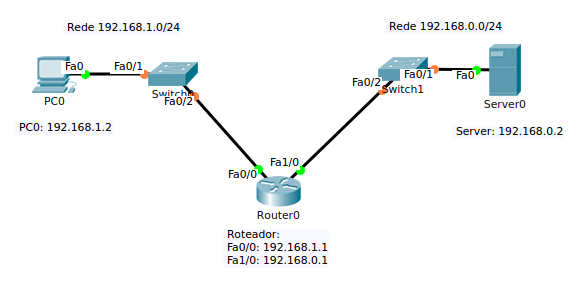
\includegraphics[scale=0.8]{figuras/figura_exemplo.png}
  \caption{Exemplo do uso de figuras no latex.}
  \label{fig:minhafigura}
\end{figure}

Segue um exemplo de como adicionar e referenciar tabelas no texto.

A Tabela \ref{tab:cenarioenderecos} apresenta as configurações de endereçamento dos nós da rede, isto é, a configuração dos hospedeiros e dos dispositivos de interconexão.

\begin{table}[!htb]
\centering
\caption{Configuração de endereçamento das interfaces dos dispositivos de rede do Cenário 1}
\label{tab:cenarioenderecos}
\footnotesize   %%diminuir tamanho do fonte (-2)
%\small          %%diminuir tamanho de fonte (-1)
\begin{tabular}{l|lll}
\toprule
& \textbf{Endereço IP} & \textbf{Máscara de Rede} & \textbf{Gateway}\\ 
\midrule
\textbf{PC0} & 192.168.1.2 & 255.255.255.0 & 192.168.1.1 \\
\textbf{Router0 - Fa0/0} & 192.168.1.1 & 255.255.255.0 & - \\
\textbf{Router0 - Fa1/0} & 192.168.0.1 & 255.255.255.0 & - \\
\textbf{Server0} & 192.168.0.2 & 255.255.255.0 & 192.168.0.1 \\
 \bottomrule
\end{tabular}
\end{table}

\subsection{Nonononono}
 Teste de referência \cite{talbot2012}.
 
\section{Discussão dos Resultados}
\label{sec:discussao}

\section{Conclusões}
\label{sec:conclusoes}

% ----------------------------------------------------------
% ELEMENTOS PÓS-TEXTUAIS
% ----------------------------------------------------------
\postextual
% ----------------------------------------------------------
% Referências bibliográficas
% ----------------------------------------------------------
\renewcommand{\bibsection}{%
\section{\bibname}
\bibmark
%\ifnobibintoc\else
%\phantomsection
%\addcontentsline{toc}{section}{\bibname}
%\fi
\prebibhook}

\bibliography{abntex2-modelo-references}



% ----------------------------------------------------------
% Apêndices
% ----------------------------------------------------------

% ---
% Inicia os apêndices
% ---
\begin{apendicesenv}

% ----------------------------------------------------------
\section*{Apêndice A - Nome do Apêndice}
\addcontentsline{toc}{section}{Apêndice A - Nome do Apêndice}
% ----------------------------------------------------------

\end{apendicesenv}
% ---


% ----------------------------------------------------------
% Anexos
% ----------------------------------------------------------

% ---
% Inicia os anexos
% ---
\begin{anexosenv}

% ---
\section*{Anexo A - Nome do Anexo}
\addcontentsline{toc}{section}{Anexo A - Nome do Anexo}
% ---
\end{anexosenv}


\end{document}
